\section{Perspektivering} \label{sec:perspektivering}
I dette afsnit perspektiveres projektet for at reflektere over de forskellige aspekter, der bør undersøges for at kunne skabe et færdigudviklet produkt, som kan anvendes af ALS-patienter. 

Systemet er udviklet til at kunne hjælpe ALS-patienter ved at aflaste deres muskler omkring knæet under en squat-øvelse. Der er ikke udviklet en prototype af et exoskelet, der muliggør dette, hvorfor systemet skal videreudvikles, således det er anvendeligt uden at være til gene for brugeren. Et eksempel på en sådan prototype fremgår af \autoref{fig:exoskelet}, hvor der ses et exoskelet påsat omkring knæet. Når muskelaktiviten er enten stigende eller faldende, vil knæets vinkel kunne sænkes eller øges ved en motor, der skal kunne styre exoskelettet.

Herudover vil det være fordelagtigt, hvis der sendes en advarsel til brugeren af systemet inden grænserne på $90^{\circ}$ og $180^{\circ}$ overskrides. Dette kan gøres ved vibration eller lyd, så brugeren ikke er påkrævet til se på exoskelettet for eksempelvis en indikation ved overstræk af knæleddet. På denne måde, vil brugen af exoskelettet ikke være tydelig for alle omkring brugeren, da det vil kunne bruges under tøj.

Brugeren skal på nuværende tidspunkt selv starte og stoppe systemet, hvilket ikke er ideelt til daglig brug af et exoskelet. Dette vil kunne videreudvikles til en funktion, som registrerer, når brugeren udfører en bevægelse. Dette vil kunne skabe det interrupt, der på nuværende tidspunkt skabes af PSoC'ens user button og igangsætter systemet. 

\begin{figure}[H]
\centering
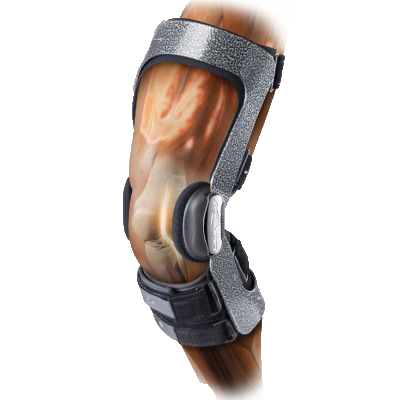
\includegraphics[width=0.5\textwidth]{figures/exoskelet}
\caption{Et exoskelet omkring knæet for at støtte den omkringliggende muskulator som hjælp til ALS-patienter \citep{djo}.}
\label{fig:exoskelet}
\end{figure}

\noindent
Herudover kan sammenhængen mellem de forskellige muskler i benet undersøges, således det vil være muligt at bevæge sig under $90^{\circ}$. Dette vil gøre systemet mere brugbart, da brugere af systemet på nuværende tidspunkt ikke kan få hjælp til at sætte sig ned i en vinkel på under $90^{\circ}$. På denne måde, vil det ikke være nødvendigt at benytte accelerometre til systemet, da EMG-målinger fra flere muskler i benet vil kunne benyttes til vurdere, om knæet flekser eller ekstenderer fra $0-180^{\circ}$.

Ud over ovennævnte kan det undersøges, hvordan mikrokontrolleren kan anvendes til opsætning af BLE-kommunikation, som det fremgår af det oprindelige design, da der i det implementerde system anvendes gumsticks til BLE-kommunkation. Disse vil ikke være nødvendige, og systemet vil derfor fylde mindre, hvis det samme kan gøres på mikrokontrolleren. 

\subsection{Et ideelt system}
Systemet vil kunne videreudvikles, således at ALS-patienter vil kunne anvende det under gang i sygdommens første stadier, og derved støtte deres muskulatur, da det på nuværende tidspunkt kun er muligt at udføre en squat-øvelse. Dette skaber ikke den mængde frihed for ALS-patienter, som det vil kunne ønskes, da det skaber begrænsninger for brugerens bevægelighed. I forhold til brugerens sikkerhed vil det kunne udvikles, så en alarm vil starte i tilfælde af, at brugeren mister balancen eller falder under gang. %\fxnote{kan godt skrive her, hvad der skal gøres ekstra - større vinkel range, flere g i accelerometre, men vil vi ikke hellere have det med til eksamen som videre udvikling af systemet? synes perspektiveringen er ret dækkende, som den er nu.}




